
\documentclass[10pt,twocolumn,letterpaper]{article}

\usepackage[pagenumbers]{cvpr} %
\usepackage{multirow}
\usepackage{multicol}
\usepackage{pgfplots}
\usepackage{svg}
\usepackage{tikz}
\usepackage{xcolor}
\usepackage{overpic}
\usetikzlibrary{calc,patterns,angles,quotes}
\usepackage{pgfplots,gincltex}
\pgfplotsset{compat=1.18}
\usepgfplotslibrary{colormaps}
\usepackage{tikz-3dplot}
\pgfplotsset{compat=newest}
%
% --- inline annotations
%
\newcommand{\red}[1]{{\color{red}#1}}
\newcommand{\todo}[1]{{\color{red}#1}}
\newcommand{\TODO}[1]{\textbf{\color{red}[TODO: #1]}}
% --- disable by uncommenting  
% \renewcommand{\TODO}[1]{}
% \renewcommand{\todo}[1]{#1}



\newcommand{\VLM}{LVLM\xspace} 
\newcommand{\ours}{PeKit\xspace}
\newcommand{\yollava}{Yo’LLaVA\xspace}

\newcommand{\thisismy}{This-Is-My-Img\xspace}
\newcommand{\myparagraph}[1]{\noindent\textbf{#1}}
\newcommand{\vdoro}[1]{{\color[rgb]{0.4, 0.18, 0.78} {[V] #1}}}
% --- disable by uncommenting  
% \renewcommand{\TODO}[1]{}
% \renewcommand{\todo}[1]{#1}
\usepackage{slashbox}
% Vectors
\newcommand{\bB}{\mathcal{B}}
\newcommand{\bw}{\mathbf{w}}
\newcommand{\bs}{\mathbf{s}}
\newcommand{\bo}{\mathbf{o}}
\newcommand{\bn}{\mathbf{n}}
\newcommand{\bc}{\mathbf{c}}
\newcommand{\bp}{\mathbf{p}}
\newcommand{\bS}{\mathbf{S}}
\newcommand{\bk}{\mathbf{k}}
\newcommand{\bmu}{\boldsymbol{\mu}}
\newcommand{\bx}{\mathbf{x}}
\newcommand{\bg}{\mathbf{g}}
\newcommand{\be}{\mathbf{e}}
\newcommand{\bX}{\mathbf{X}}
\newcommand{\by}{\mathbf{y}}
\newcommand{\bv}{\mathbf{v}}
\newcommand{\bz}{\mathbf{z}}
\newcommand{\bq}{\mathbf{q}}
\newcommand{\bff}{\mathbf{f}}
\newcommand{\bu}{\mathbf{u}}
\newcommand{\bh}{\mathbf{h}}
\newcommand{\bb}{\mathbf{b}}

\newcommand{\rone}{\textcolor{green}{R1}}
\newcommand{\rtwo}{\textcolor{orange}{R2}}
\newcommand{\rthree}{\textcolor{red}{R3}}
\usepackage{amsmath}
%\usepackage{arydshln}
\DeclareMathOperator{\similarity}{sim}
\DeclareMathOperator{\AvgPool}{AvgPool}

\newcommand{\argmax}{\mathop{\mathrm{argmax}}}     



\definecolor{cvprblue}{rgb}{0.21,0.49,0.74}
\definecolor{lightboldcolor}{gray}{0.6}
\usepackage[pagebackref,breaklinks,colorlinks,allcolors=cvprblue]{hyperref}

\newcommand{\ZL}[1]{{ \color{magenta}{ ZL: #1 }}}
\newcommand{\HZ}[1]{{ \color{cyan}{HZ: #1}}}
\newcommand{\lightbold}[1]{\textbf{\textcolor{lightboldcolor}{#1}}}


\def\paperID{12874} %
\def\confName{CVPR}
\def\confYear{2025}

\title{Laplace-Beltrami Operator for Gaussian Splatting}
\author{Hongyu Zhou$^{1,2}$ \qquad\qquad Zorah Lähner$^{1,2}$ \\
\ \\
$^1$University of Bonn \qquad \qquad $^2$Lamarr Institute\\
{\tt\small hzhou,laehner@uni-bonn.de}
}

\begin{document}

\twocolumn[{%
\renewcommand\twocolumn[1][]{#1}%
\maketitle
\begin{center}
    \centering
    \captionsetup{type=figure}
    \includegraphics[width=1.0\textwidth,height=4.6cm]{figures/teaser.png}
    \captionof{figure}{We introduce a novel method to accurately compute the Laplace-Beltrami operator directly on 3D Gaussian splats, leveraging both the center and the covariance information. The operator can be directly applied on 3D Gaussian splats, without the need for mesh extraction, for multiple applications such as surface smoothing, as shown above. We can transform the original scene (left) by computing the Laplace-Beltrami eigenfunctions (middle, both original and smoothed), leading to a smoothed scene of the 3D Gaussians splats (right), which presents transformation on the original rendering (left) and the computed Laplace-Beltrami eigenfunction (middle). %
\label{fig:teaser}}
\end{center}%
}]

\begin{abstract}


The choice of representation for geographic location significantly impacts the accuracy of models for a broad range of geospatial tasks, including fine-grained species classification, population density estimation, and biome classification. Recent works like SatCLIP and GeoCLIP learn such representations by contrastively aligning geolocation with co-located images. While these methods work exceptionally well, in this paper, we posit that the current training strategies fail to fully capture the important visual features. We provide an information theoretic perspective on why the resulting embeddings from these methods discard crucial visual information that is important for many downstream tasks. To solve this problem, we propose a novel retrieval-augmented strategy called RANGE. We build our method on the intuition that the visual features of a location can be estimated by combining the visual features from multiple similar-looking locations. We evaluate our method across a wide variety of tasks. Our results show that RANGE outperforms the existing state-of-the-art models with significant margins in most tasks. We show gains of up to 13.1\% on classification tasks and 0.145 $R^2$ on regression tasks. All our code and models will be made available at: \href{https://github.com/mvrl/RANGE}{https://github.com/mvrl/RANGE}.

\end{abstract}

    
\section{Introduction}
Backdoor attacks pose a concealed yet profound security risk to machine learning (ML) models, for which the adversaries can inject a stealth backdoor into the model during training, enabling them to illicitly control the model's output upon encountering predefined inputs. These attacks can even occur without the knowledge of developers or end-users, thereby undermining the trust in ML systems. As ML becomes more deeply embedded in critical sectors like finance, healthcare, and autonomous driving \citep{he2016deep, liu2020computing, tournier2019mrtrix3, adjabi2020past}, the potential damage from backdoor attacks grows, underscoring the emergency for developing robust defense mechanisms against backdoor attacks.

To address the threat of backdoor attacks, researchers have developed a variety of strategies \cite{liu2018fine,wu2021adversarial,wang2019neural,zeng2022adversarial,zhu2023neural,Zhu_2023_ICCV, wei2024shared,wei2024d3}, aimed at purifying backdoors within victim models. These methods are designed to integrate with current deployment workflows seamlessly and have demonstrated significant success in mitigating the effects of backdoor triggers \cite{wubackdoorbench, wu2023defenses, wu2024backdoorbench,dunnett2024countering}.  However, most state-of-the-art (SOTA) backdoor purification methods operate under the assumption that a small clean dataset, often referred to as \textbf{auxiliary dataset}, is available for purification. Such an assumption poses practical challenges, especially in scenarios where data is scarce. To tackle this challenge, efforts have been made to reduce the size of the required auxiliary dataset~\cite{chai2022oneshot,li2023reconstructive, Zhu_2023_ICCV} and even explore dataset-free purification techniques~\cite{zheng2022data,hong2023revisiting,lin2024fusing}. Although these approaches offer some improvements, recent evaluations \cite{dunnett2024countering, wu2024backdoorbench} continue to highlight the importance of sufficient auxiliary data for achieving robust defenses against backdoor attacks.

While significant progress has been made in reducing the size of auxiliary datasets, an equally critical yet underexplored question remains: \emph{how does the nature of the auxiliary dataset affect purification effectiveness?} In  real-world  applications, auxiliary datasets can vary widely, encompassing in-distribution data, synthetic data, or external data from different sources. Understanding how each type of auxiliary dataset influences the purification effectiveness is vital for selecting or constructing the most suitable auxiliary dataset and the corresponding technique. For instance, when multiple datasets are available, understanding how different datasets contribute to purification can guide defenders in selecting or crafting the most appropriate dataset. Conversely, when only limited auxiliary data is accessible, knowing which purification technique works best under those constraints is critical. Therefore, there is an urgent need for a thorough investigation into the impact of auxiliary datasets on purification effectiveness to guide defenders in  enhancing the security of ML systems. 

In this paper, we systematically investigate the critical role of auxiliary datasets in backdoor purification, aiming to bridge the gap between idealized and practical purification scenarios.  Specifically, we first construct a diverse set of auxiliary datasets to emulate real-world conditions, as summarized in Table~\ref{overall}. These datasets include in-distribution data, synthetic data, and external data from other sources. Through an evaluation of SOTA backdoor purification methods across these datasets, we uncover several critical insights: \textbf{1)} In-distribution datasets, particularly those carefully filtered from the original training data of the victim model, effectively preserve the model’s utility for its intended tasks but may fall short in eliminating backdoors. \textbf{2)} Incorporating OOD datasets can help the model forget backdoors but also bring the risk of forgetting critical learned knowledge, significantly degrading its overall performance. Building on these findings, we propose Guided Input Calibration (GIC), a novel technique that enhances backdoor purification by adaptively transforming auxiliary data to better align with the victim model’s learned representations. By leveraging the victim model itself to guide this transformation, GIC optimizes the purification process, striking a balance between preserving model utility and mitigating backdoor threats. Extensive experiments demonstrate that GIC significantly improves the effectiveness of backdoor purification across diverse auxiliary datasets, providing a practical and robust defense solution.

Our main contributions are threefold:
\textbf{1) Impact analysis of auxiliary datasets:} We take the \textbf{first step}  in systematically investigating how different types of auxiliary datasets influence backdoor purification effectiveness. Our findings provide novel insights and serve as a foundation for future research on optimizing dataset selection and construction for enhanced backdoor defense.
%
\textbf{2) Compilation and evaluation of diverse auxiliary datasets:}  We have compiled and rigorously evaluated a diverse set of auxiliary datasets using SOTA purification methods, making our datasets and code publicly available to facilitate and support future research on practical backdoor defense strategies.
%
\textbf{3) Introduction of GIC:} We introduce GIC, the \textbf{first} dedicated solution designed to align auxiliary datasets with the model’s learned representations, significantly enhancing backdoor mitigation across various dataset types. Our approach sets a new benchmark for practical and effective backdoor defense.



\section{Related Work}
In this section, we show connections to the most relevant related work. A broader introduction into Gaussian splatting can be found in the survey of \cite{chen2024survey3dgaussiansplatting}.

\subsection{Gaussian Splatting}\label{sub:rw:gaussian}

3D Gaussian splatting was introduced in \cite{kerbl3Dgaussians} as an efficient framework for novel-view synthesis. 
It optimizes over a set of Gaussian distributions in 3D space with color and opacity values which can be rendered from new view points. 
While this works exceptionally well and has been applied to many applications~\cite{SplattingAvatar:CVPR2024,yan2024street}, the pipeline is focused on clean-looking rendering results but not clean geometry. 
To overcome this, several methods introduced additional constrains that focus on the geometric accuracy in the optimization. 
For example, the method of \cite{Huang2DGS2024} restricts the variance to a 2D plane (the dimension of the surface). 
Another approach, SuGaR~\cite{guedon2023sugar}, extracts a mesh and realigns the Gaussian splats with the surface of this mesh to obtain a cleaner geometry. 
Gaussian opacity fields~\cite{yu2024gaussian} combine Gaussians with a signed distance function to further regularize the results. 
While this leads to better geometry, the extraction of a mesh in the process is expensive and the extracted mesh might still be noisy. Without the extraction, outlier splats can prevail, and while they tend to not deteriorate the rendering, they can heavily interfere with geometry processing applications.


\subsection{Laplacian-Beltrami Operator}\label{sub:rw:lbo}

\paragraph{Laplacian Operator on Meshes.} 
The Laplace-Beltrami operator (LBO) is the generalization of the second derivative on general manifolds and a popular tool in many geometry processing applications. 
Its discretization, especially on triangular meshes, has been studied extensively and it has been shown that not all properties of the continuous Laplacian can be fulfilled in the discrete case at the same time~\cite{wardetzky2007nofreelunch}. 
While it is possible to use the graph Laplacian~\cite{taubin1995fairsurface} on a mesh by discarding the face information, this fails to take into account all information about the local geometry. 
More advanced mesh LBOs, like the cotan discretization~\cite{pinkallporthier,meyer2003discrete} or intrinsic Delaunay discretization~\cite{bobenko2007simplicial}, provide a more accurate approximation of the continuous behaviour. 
These can also be extended to more complex domains, like n-dimensional data~\cite{crane2019ndim}, general polygonal meshes~\cite{alexa2011polygonal,bunge2020polygon}, or non-manifold meshes~\cite{sharp2020nonmanifold}.
However, all of these depend on explicitly given connectivity information which can guarantee certain properties but does not work for less structured shape representations, like point clouds or Gaussian splatting.

\paragraph{Laplacian Operator on Point Clouds.} 
As the discrete Laplacian operator relies on the definition of the neighborhood that is not explicitly given in the point cloud, it is essential to estimate the neighborhood function in a good way so that it approximate the intrinsic connectivity.
A straight-forward solution would be to triangulate the point cloud, however, this is expensive and often leads to errors on sparse or noisy point clouds. 
Instead, a common solution is to \emph{locally} approximate the surface via its tangent plane and projection of surrounding points onto it, often by a nearest neighbor search~\cite{Belkin2009ConstructingLO}. 
This works well on smooth or flat regions, but struggles around very sharp features. 
The resulting inaccuracies can be diminished by building an operator that is robust to incorrectly found and non-manifold surface connections~\cite{sharp2020nonmanifold}, or by 
employing improvements in the surface estimation for these cases, for example through anisotropic Voronoi diagrams~\cite{Qin2018anisotropic}, or physic dynamics~\cite{petronetto2013meshfree}.
The recent work of \cite{pang2024neurallaplacianoperator3d} avoids direct estimation of the surface by learning the behavior of the LBO on different examples and then generalizing the behavior directly to new point clouds. 
While the centers of a Gaussian splatting do form a point cloud on which the previous methods can be applied, the directional variance at each point provides valuable additional information about the surface. 
In this work we propose a more accurate way to extract the LBO from Gaussian splatting which includes the variances in the surface estimation. 



\section{Background}
\label{sec:background}

In this section we introduce the background on Gaussian splatting and the Laplace-Beltrami operator necessary to understand the rest of the paper. 

\subsection{Gaussian Splatting} \label{sub:bg:gaussian}

3D Gaussian splatting~\cite{kerbl3Dgaussians} represents a scene as a collection of 3D Gaussian distributions $\{ (\mu_i, \Sigma_i, \alpha_i, c_i) \}_i$ with mean $\mu_i \in \mathbb{R}^3$, variance $\Sigma_i \in \mathbb{R}^{3 \times 3}$, alpha value $\alpha_i$, and color function $c_i$ in spherical harmonic representation. 
This collection can be easily projected to 2D and rendered by accumulating density along a ray. 
The parameters of each Gaussian splat are optimized to render to a set of training images from different view points. 
Since this optimization is focused on rendering, the 3D Gaussian splats are not necessarily localized on the surface of the objects in the scene. 
There have been efforts to align the 3D Gaussian splats to the surface by regularizing on the SDF~\cite{guedon2023sugar}, the depth and the normal~\cite{yu2024gaussian}, or training 2D Gaussian splatting~\cite{Huang2DGS2024}, that focus on the geometry of the reconstructed mesh.

\subsection{(Discrete) Laplace-Beltrami Operator} \label{sub:bg:lbo}

The Laplace-Beltrami operator (LBO) $L = \text{div}\cdot \nabla$ generalizes the second derivative to general closed compact manifolds. 
The operator and its eigenfunctions and eigenvalues, which are non-trivial solutions to $L \phi_i = \lambda_i \phi_i$, are popular tools in geometry processing (see \cref{sub:rw:lbo}). 
When discretizing the underlying manifold, the LBO also has to be discretized which leads to approximation artifacts \cite{wardetzky2007nofreelunch}. 

\begin{figure}
    \centering
    (a) 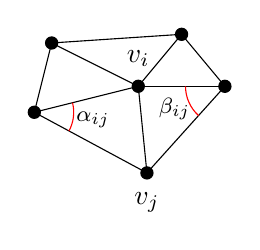
\begin{tikzpicture}[scale=1.1]
    \coordinate (i) at (0,0);
    \coordinate (A) at (1,0);
    \coordinate (B) at (0.5,0.6);
    \coordinate (C) at (-1,0.5);
    \coordinate (D) at (-1.2,-0.3);
    \coordinate (E) at (0.1,-1);

    \node[label=below:{$v_j$}] (EN) at (E) {};
    \node[label=above:{$v_i$}] (iN) at (i) {};

    \draw (i) -- (A);
    \draw (i) -- (B);
    \draw (i) -- (C);
    \draw (i) -- (D);
    \draw (i) -- (E);

    \draw (A) -- (B);
    \draw (B) -- (C);
    \draw (C) -- (D);
    \draw (D) -- (E);
    \draw (E) -- (A);

    \pic [draw=red, -, "\footnotesize{$\alpha_{ij}$}", angle eccentricity=1.5] {angle = E--D--i};
    \pic [draw=red, -, "\footnotesize{$\beta_{ij}$}", angle eccentricity=1.4] {angle = i--A--E};
       
      
    \draw[fill=black, draw=black] (i) circle (2pt);
    \draw[fill=black, draw=black] (A) circle (2pt);
    \draw[fill=black, draw=black] (B) circle (2pt);
    \draw[fill=black, draw=black] (C) circle (2pt);
    \draw[fill=black, draw=black] (D) circle (2pt);
    \draw[fill=black, draw=black] (E) circle (2pt);
\end{tikzpicture}

    (b) \includegraphics[width=.4\linewidth]{figures/projection.png}
    \caption{Discretization of the Laplace Beltrami operator on a mesh (a) and a point cloud (b). In the mesh the connectivity is directly given and can be used to compute properties like angles. The point cloud Laplacian relies on a approximation of tangent plane at a point on which the neighborhood is projected (blue). }
    \label{fig:cotan}
\end{figure}

The cotan-discretization \cite{pinkallporthier} for triangular meshes is defined as follows:
\begin{align}
    W_{ij} = \begin{cases}
        \frac{1}{2} (\text{cot}\alpha_{ij} + \text{cot} \beta_{ij}), & \text{if } (i,j) \in E \\
        - \sum_{k \in \mathcal{N}(i)} w_{ik}, & \text{if } j=i \\
        0, & \text{otherwise}
    \end{cases}
\end{align}
where $\alpha_{ij}, \beta_{ij}$ are the opposing angles to the edge between vertices $v_i, v_j$ (see \cref{fig:cotan}). 
In combination with the diagonal mass matrix $M$ describing the local weight at each vertex $M_{ii}$ the area of the voronoi cell around vertex $i$, the LBO is $L = M^{-1} W$.
While the default cotan-Laplacian does not fulfill the maximum principle, it will when applied to the intrinsic Delaunay triangulation of the input mesh \cite{bobenko2007simplicial}.
However, this depends on a clean mesh with only triangles and no non-manifoldness (e.g., edges with three triangles attached). 
For meshes of arbitrary topology, \cite{sharp2020nonmanifold} suggested to use the tufted cover, which generates an implicit manifold overlay of a given connectivity, in combination with the intrinsic triangulation. 
Due to its flexibility w.r.t. the connectivity, the tufted Laplacian is also well-suited to be used on point clouds by approximating a local neighborhood and connectivity for each point without the need to reconstruct a full, consistent triangle mesh, which is expensive and prone to be noisy. 

\section{Methodology}

\subsection{Problem Definition}

Given a multivariate time series input $X \in \mathbb{R}^{C  \times T}$, multivariate time series forecasting tasks are designed to predict its future $F$ time steps $\hat{Y}\in \mathbb{R}^{C \times F}$ using past $T$ steps. $C $ is the number of variates or channels.

\subsection{Preliminary Analysis}

This section presents why RevIN~\citep{Kim_revin,liu2022non}, High-pass, and Low-pass filters fail to address the Mid-Frequency Spectrum Gap. Let the input univariate time series be $ x(t) $ with length $ T $ and target $ y(t) $ with length $ F $. 

\begin{definition}[Frequency Spectral Energy]\label{def:energy}
The Fourier transform of $x(t)$, $X(f)$, and its spectral energy $E_X(f)$ is given by:
\vspace{-0.2cm}
\begin{align}
X(f) = \sum_{t=0}^{T-1} x(t) e^{-i 2 \pi f t / {T-1}}, \quad &f = 0, 1, \dots, T-1\notag\\
E_X(f) = |X(f)|^2.
\end{align}
\vspace{-0.2cm}
\end{definition}

\textbf{Impact of RevIN on Frequency Spectrum \quad}
\begin{definition}[Reversible Instance Normalization]\label{def:RevIN}
Given a \textbf{forecast model} $ f: \mathbb{R}^T \rightarrow \mathbb{R}^F $ that generates a forecast $ \hat{y}(t) $ from a given input $x(t)$, RevIN is defined as:
\vspace{-0.2cm}
\begin{align}
&\hat{x}(t) = \frac{x(t) - \mu}{\sigma},\quad t = 0, 1, \dots, T-1\notag\\
&\hat{y}(t) = f(\hat{x}(t)), \quad \hat{y}(t)_{rev}= \hat{y}(t) \cdot \sigma + \mu,\notag\\
&\mu = \frac{1}{T} \sum_{t=0}^{T-1} x(t), \quad \sigma = \sqrt{\frac{1}{T} \sum_{t=0}^{T-1} (x(t) - \mu)^2}.
\end{align}
\vspace{-0.2cm}
\end{definition}

\begin{theorem} [Frequency Spectrum after RevIN] \label{theorem:RevIN}
\vspace{-0.2cm}
The spectral energy of $\hat{x}(t)$ (transformed using RevIN):
\begin{align}
E_{\hat{X}}(0)=0,& \quad f=0, \notag\\
E_{\hat{X}}(f) = \left( \frac{1}{\sigma} \right)^2 |X(f)|^2,&\quad f = 1,2,\dots, T-1 . 
\end{align}
\vspace{-0.2cm}
\end{theorem}
The proof is in Appendix~\ref{app:RevIN}. Theorem~\ref{theorem:RevIN} suggests that RevIN scales the absolute spectral energy by $ \sigma^2 $ but does not affect its relative distribution except $E_{\hat{X}}(0)=0$. Thus, RevIN preserves the relative spectral energy distribution and leaves the Mid-Frequency Spectrum Gap unresolved. \textit{However, our experiments still employ RevIN to ensure a fair comparison with other baselines.}
\begin{figure*}[h]
  \centering
  \includegraphics[width=1.\linewidth]{Faker/source/assets/jpg/ReFocus.jpg}
  \caption{General structure of \textbf{ReFocus}. `Adaptive Mid-Frequency Energy Optimizer (AMEO)' enhances mid-frequency components modeling, and `Energy-based Key-Frequency Picking Block' (EKPB) effectively captures shared Key-Frequency across channels}
  \label{fig:refocus}
\end{figure*}

\begin{figure*}[h]
  \centering
  \includegraphics[width=0.7\linewidth]{Faker/source/assets/jpg/ket.jpg}
  \caption{General process of the \textbf{Key-Frequency Enhanced Training strategy (KET)}, where spectral information from other channels is randomly introduced into each channel, to enhance the extraction of the shared Key-Frequency.}
  \label{fig:reshuffle}
\end{figure*}
\textbf{Impact of High- and Low-pass filter \quad}
We still define $\hat{x}(t)$ to be the filtered (processed) signal, obtained by applying a filter $H(f)$ (High/Low-pass filter). The filter $ H(f) $ is 1 in the passband (High/Low frequency) and 0 in the stopband (Middle frequency). So $E_{\hat{X}}(f)=0,\quad E_{\hat{X}}\leq E_X(f)$ for middle frequencies, which creates even larger gap.

\subsection{Overall Structure of The Proposed ReFocus}

In this section, we elucidate the overall architecture of \textbf{ReFocus}, depicted in Figure \ref{fig:refocus}. We define frequency domain projection as $D1\rightarrow D2$ representing a projection from dimension $D1$ to $D2$ in the frequency domain~\citep{xu2024fits}. Initially, we apply \textbf{AMEO} to the input $X \in \mathbb{R}^{C \times T}$, yielding the processed spectrum $ X_{am} \in \mathbb{R}^{C  \times T} $. Next, we use a projection $T\rightarrow D$ to transform $ X_{am}$ into the Variate Embedding $ X_{em} \in \mathbb{R}^{C  \times D}$~\citep{LiuiTransformer}. Then, $X_{em}$ go through $N$ \textbf{EKPB} to generate representation $H_{N+1}$, which is projected to obtain final prediction $\hat{Y}$. 

\textbf{Adaptive Mid-Frequency Energy Optimizer \quad}
Building upon the \textbf{Preliminary Analysis}, we propose a convolution- and residual learning-based solution to address the Mid-Frequency Spectrum Gap, which we denoted as AMEO. 
\begin{definition}[Adaptive Mid-Frequency Energy Optimizer]\label{def:AMEO}
AMEO is defined as:
\begin{align}
&\hat{x}(t) = x(t)-\frac{\beta}{K}\sum_{k=0}^{K-1} \tilde{x}(t+K-1-k),\notag\\
&\tilde{x}(t) =\notag\\
&\begin{cases}
x(t-(\frac{K}{2}+1)), \quad \text{if } \frac{K}{2}+1 \leq t < T+\frac{K}{2}+1, \\
0,  \quad\text{if } 0 \leq t < \frac{K}{2}+1 \text{ or } T+\frac{K}{2}+1 \leq t < T+K.
\end{cases}
\end{align}
\vspace{-0.2cm}
\end{definition}

It is equivalent to $x=x-\beta \cdot Conv(x)$. $Conv$ is a 1D convolution (Zero-padding at both ends, stride $s=1$, kernel size $K$, with values initialized as $ \frac{1}{K} $). $\beta \in \mathbb{R}^{1}$ is a hyperparameter.

\begin{theorem} [Frequency Spectrum after AMEO] \label{theorem:AMEO}
The spectral energy of $\hat{x}(t)$ obtained using AMEO:
\begin{align}
E_{\hat{X}}(f) =|X(f)|^2 \left\{1 - \beta \cdot \underbrace{\frac{1}{K} \sum_{k=0}^{K-1} e^{i 2 \pi f (\frac{3K}{2}-k -2) / {T-1}}}_{G(f)}\right\}^2
\end{align}
\vspace{-0.2cm}
\end{theorem}

The proof is in Appendix~\ref{app:AMEO}. We have $E_{\hat{X}}(f) =|X(f)|^2(1-\beta  \cdot G(f))^2$. Generally, $ G(f) $ behaves as a decay function, gradually reducing its value from \textbf{One} to \textbf{Zero}. Such \textbf{decay behavior} makes AMEO relatively enhances mid-frequency components, thus addressing the Mid-Frequency Spectrum Gap.

\textbf{Energy-based Key-Frequency Picking Block \quad} In each \textbf{EKPB}, the input $ H_i \in \mathbb{R}^{C  \times D} (H_1=X_{em}) $ is first processed through an MLP to generate $ H_i^k \in \mathbb{R}^{C  \times Q}$. Then, FFT is applied to get $ H_i^f \in \mathbb{R}^{C  \times (Q/2+1)}$. For $ H_i^f$, we calculate its energy, denoted as $ H_i^e \in \mathbb{R}^{C  \times (Q/2+1)}$. A cross-channel softmax is then applied to $ H_i^e$ per frequency to obtain a probability distribution $ H_i^{soft} \in \mathbb{R}^{C  \times (Q/2+1)}$. Using $H_i^{soft}$, we select values from $ H_i^f$ across channels for each frequency, resulting in $K^f_i \in \mathbb{R}^{1  \times (Q/2+1)}$, which represents the Shared Key-Frequency across all channels. Then iFFT is performed on $K^f_i$ to get $K_i\in \mathbb{R}^{1  \times Q}$, followed by projection $Q\rightarrow D$ and repeating (C times) to get $\hat{K}_i \in \mathbb{R}^{C  \times D}$. This $\hat{K}_i$ is point-wisely added to $\hat{H_i}\in \mathbb{R}^{C  \times D}$ , which is the projection of $ H_i$ using projection $D\rightarrow D$. Then, an MLP and $Add\&Norm$ is applied to the result $HK\in \mathbb{R}^{C  \times D}$ to fuse inter-series dependencies information, and another MLP and $Add\&Norm$ is used to capture intra-series variations~\citep{LiuiTransformer}. The output of each \textbf{EKPB} is $\hat{O_i} \in \mathbb{R}^{C  \times D}$, where $H_{i+1}=\hat{O_i}$.

\subsection{Key-Frequency Enhanced Training strategy}

In real-world time series, certain channels often exhibit spectral dependencies, which may not be fully captured in the training set, and the specific channels with such dependencies are also unknown~\citep{geweke1984freqchannel,Zhao2024freqchannel}. So this work borrows insight from recent advancement of mix-up in time series~\citep{zhou2023mixup,ansari2024mixup}, randomly introducing spectral information from other channels into each channel, to enhance the extraction of the shared Key-Frequency, as in Figure~\ref{fig:reshuffle}. Given a multivariate time series input $X \in \mathbb{R}^{C \times T}$ and its ground-truth $Y \in \mathbb{R}^{C \times F}$, we generate a pseudo sample pair: 

\begin{align}
X' = iFFT(FFT(X) +\alpha \cdot FFT(X[\text{perm},:]))&,  \notag\\ 
Y' = iFFT(FFT(Y) +\alpha \cdot FFT(Y[\text{perm},:]))&.
\end{align}

$\alpha \in \mathbb{R}^{C \times 1}$ is a weight vector sampled from a normal distribution, $\text{perm}$ is a reshuffled channel index. Since $FFT$ and $iFFT$ are linear operations, this mix-up process can be equivalently simplified in the \textbf{Time Domain}:
\begin{align}
X' = X +\alpha \cdot X[\text{perm},:]&,  \notag\\
Y' = Y +\alpha \cdot Y[\text{perm},:]&
 \end{align}
We alternate training between real and synthetic data to preserve the spectral dependencies in real samples. This combines the advantages of data augmentation, such as improved generalization, while mitigating potential drawbacks like over-smoothing and training instability~\citep{ryu2024tf,alkhalifah2022tf}.












\section{Experiments}

\subsection{Setups}
\subsubsection{Implementation Details}
We apply our FDS method to two types of 3DGS: 
the original 3DGS, and 2DGS~\citep{huang20242d}. 
%
The number of iterations in our optimization 
process is 35,000.
We follow the default training configuration 
and apply our FDS method after 15,000 iterations,
then we add normal consistency loss for both
3DGS and 2DGS after 25000 iterations.
%
The weight for FDS, $\lambda_{fds}$, is set to 0.015,
the $\sigma$ is set to 23,
and the weight for normal consistency is set to 0.15
for all experiments. 
We removed the depth distortion loss in 2DGS 
because we found that it degrades its results in indoor scenes.
%
The Gaussian point cloud is initialized using Colmap
for all datasets.
%
%
We tested the impact of 
using Sea Raft~\citep{wang2025sea} and 
Raft\citep{teed2020raft} on FDS performance.
%
Due to the blurriness of the ScanNet dataset, 
additional prior constraints are required.
Thus, we incorporate normal prior supervision 
on the rendered normals 
in ScanNet (V2) dataset by default.
The normal prior is predicted by the Stable Normal 
model~\citep{ye2024stablenormal}
across all types of 3DGS.
%
The entire framework is implemented in 
PyTorch~\citep{paszke2019pytorch}, 
and all experiments are conducted on 
a single NVIDIA 4090D GPU.

\begin{figure}[t] \centering
    \makebox[0.16\textwidth]{\scriptsize Input}
    \makebox[0.16\textwidth]{\scriptsize 3DGS}
    \makebox[0.16\textwidth]{\scriptsize 2DGS}
    \makebox[0.16\textwidth]{\scriptsize 3DGS + FDS}
    \makebox[0.16\textwidth]{\scriptsize 2DGS + FDS}
    \makebox[0.16\textwidth]{\scriptsize GT (Depth)}

    \includegraphics[width=0.16\textwidth]{figure/fig3_img/compare3/gt_rgb/frame_00522.jpg}
    \includegraphics[width=0.16\textwidth]{figure/fig3_img/compare3/3DGS/frame_00522.jpg}
    \includegraphics[width=0.16\textwidth]{figure/fig3_img/compare3/2DGS/frame_00522.jpg}
    \includegraphics[width=0.16\textwidth]{figure/fig3_img/compare3/3DGS+FDS/frame_00522.jpg}
    \includegraphics[width=0.16\textwidth]{figure/fig3_img/compare3/2DGS+FDS/frame_00522.jpg}
    \includegraphics[width=0.16\textwidth]{figure/fig3_img/compare3/gt_depth/frame_00522.jpg} \\

    % \includegraphics[width=0.16\textwidth]{figure/fig3_img/compare1/gt_rgb/frame_00137.jpg}
    % \includegraphics[width=0.16\textwidth]{figure/fig3_img/compare1/3DGS/frame_00137.jpg}
    % \includegraphics[width=0.16\textwidth]{figure/fig3_img/compare1/2DGS/frame_00137.jpg}
    % \includegraphics[width=0.16\textwidth]{figure/fig3_img/compare1/3DGS+FDS/frame_00137.jpg}
    % \includegraphics[width=0.16\textwidth]{figure/fig3_img/compare1/2DGS+FDS/frame_00137.jpg}
    % \includegraphics[width=0.16\textwidth]{figure/fig3_img/compare1/gt_depth/frame_00137.jpg} \\

     \includegraphics[width=0.16\textwidth]{figure/fig3_img/compare2/gt_rgb/frame_00262.jpg}
    \includegraphics[width=0.16\textwidth]{figure/fig3_img/compare2/3DGS/frame_00262.jpg}
    \includegraphics[width=0.16\textwidth]{figure/fig3_img/compare2/2DGS/frame_00262.jpg}
    \includegraphics[width=0.16\textwidth]{figure/fig3_img/compare2/3DGS+FDS/frame_00262.jpg}
    \includegraphics[width=0.16\textwidth]{figure/fig3_img/compare2/2DGS+FDS/frame_00262.jpg}
    \includegraphics[width=0.16\textwidth]{figure/fig3_img/compare2/gt_depth/frame_00262.jpg} \\

    \includegraphics[width=0.16\textwidth]{figure/fig3_img/compare4/gt_rgb/frame00000.png}
    \includegraphics[width=0.16\textwidth]{figure/fig3_img/compare4/3DGS/frame00000.png}
    \includegraphics[width=0.16\textwidth]{figure/fig3_img/compare4/2DGS/frame00000.png}
    \includegraphics[width=0.16\textwidth]{figure/fig3_img/compare4/3DGS+FDS/frame00000.png}
    \includegraphics[width=0.16\textwidth]{figure/fig3_img/compare4/2DGS+FDS/frame00000.png}
    \includegraphics[width=0.16\textwidth]{figure/fig3_img/compare4/gt_depth/frame00000.png} \\

    \includegraphics[width=0.16\textwidth]{figure/fig3_img/compare5/gt_rgb/frame00080.png}
    \includegraphics[width=0.16\textwidth]{figure/fig3_img/compare5/3DGS/frame00080.png}
    \includegraphics[width=0.16\textwidth]{figure/fig3_img/compare5/2DGS/frame00080.png}
    \includegraphics[width=0.16\textwidth]{figure/fig3_img/compare5/3DGS+FDS/frame00080.png}
    \includegraphics[width=0.16\textwidth]{figure/fig3_img/compare5/2DGS+FDS/frame00080.png}
    \includegraphics[width=0.16\textwidth]{figure/fig3_img/compare5/gt_depth/frame00080.png} \\



    \caption{\textbf{Comparison of depth reconstruction on Mushroom and ScanNet datasets.} The original
    3DGS or 2DGS model equipped with FDS can remove unwanted floaters and reconstruct
    geometry more preciously.}
    \label{fig:compare}
\end{figure}


\subsubsection{Datasets and Metrics}

We evaluate our method for 3D reconstruction 
and novel view synthesis tasks on
\textbf{Mushroom}~\citep{ren2024mushroom},
\textbf{ScanNet (v2)}~\citep{dai2017scannet}, and 
\textbf{Replica}~\citep{replica19arxiv}
datasets,
which feature challenging indoor scenes with both 
sparse and dense image sampling.
%
The Mushroom dataset is an indoor dataset 
with sparse image sampling and two distinct 
camera trajectories. 
%
We train our model on the training split of 
the long capture sequence and evaluate 
novel view synthesis on the test split 
of the long capture sequences.
%
Five scenes are selected to evaluate our FDS, 
including "coffee room", "honka", "kokko", 
"sauna", and "vr room". 
%
ScanNet(V2)~\citep{dai2017scannet}  consists of 1,613 indoor scenes
with annotated camera poses and depth maps. 
%
We select 5 scenes from the ScanNet (V2) dataset, 
uniformly sampling one-tenth of the views,
following the approach in ~\citep{guo2022manhattan}.
To further improve the geometry rendering quality of 3DGS, 
%
Replica~\citep{replica19arxiv} contains small-scale 
real-world indoor scans. 
We evaluate our FDS on five scenes from 
Replica: office0, office1, office2, office3 and office4,
selecting one-tenth of the views for training.
%
The results for Replica are provided in the 
supplementary materials.
To evaluate the rendering quality and geometry 
of 3DGS, we report PSNR, SSIM, and LPIPS for 
rendering quality, along with Absolute Relative Distance 
(Abs Rel) as a depth quality metrics.
%
Additionally, for mesh evaluation, 
we use metrics including Accuracy, Completion, 
Chamfer-L1 distance, Normal Consistency, 
and F-scores.




\subsection{Results}
\subsubsection{Depth rendering and novel view synthesis}
The comparison results on Mushroom and 
ScanNet are presented in \tabref{tab:mushroom} 
and \tabref{tab:scannet}, respectively. 
%
Due to the sparsity of sampling 
in the Mushroom dataset,
challenges are posed for both GOF~\citep{yu2024gaussian} 
and PGSR~\citep{chen2024pgsr}, 
leading to their relative poor performance 
on the Mushroom dataset.
%
Our approach achieves the best performance 
with the FDS method applied during the training process.
The FDS significantly enhances the 
geometric quality of 3DGS on the Mushroom dataset, 
improving the "abs rel" metric by more than 50\%.
%
We found that Sea Raft~\citep{wang2025sea}
outperforms Raft~\citep{teed2020raft} on FDS, 
indicating that a better optical flow model 
can lead to more significant improvements.
%
Additionally, the render quality of RGB 
images shows a slight improvement, 
by 0.58 in 3DGS and 0.50 in 2DGS, 
benefiting from the incorporation of cross-view consistency in FDS. 
%
On the Mushroom
dataset, adding the FDS loss increases 
the training time by half an hour, which maintains the same
level as baseline.
%
Similarly, our method shows a notable improvement on the ScanNet dataset as well using Sea Raft~\citep{wang2025sea} Model. The "abs rel" metric in 2DGS is improved nearly 50\%. This demonstrates the robustness and effectiveness of the FDS method across different datasets.
%


% \begin{wraptable}{r}{0.6\linewidth} \centering
% \caption{\textbf{Ablation study on geometry priors.}} 
%         \label{tab:analysis_prior}
%         \resizebox{\textwidth}{!}{
\begin{tabular}{c| c c c c c | c c c c}

    \hline
     Method &  Acc$\downarrow$ & Comp $\downarrow$ & C-L1 $\downarrow$ & NC $\uparrow$ & F-Score $\uparrow$ &  Abs Rel $\downarrow$ &  PSNR $\uparrow$  & SSIM  $\uparrow$ & LPIPS $\downarrow$ \\ \hline
    2DGS&   0.1078&  0.0850&  0.0964&  0.7835&  0.5170&  0.1002&  23.56&  0.8166& 0.2730\\
    2DGS+Depth&   0.0862&  0.0702&  0.0782&  0.8153&  0.5965&  0.0672&  23.92&  0.8227& 0.2619 \\
    2DGS+MVDepth&   0.2065&  0.0917&  0.1491&  0.7832&  0.3178&  0.0792&  23.74&  0.8193& 0.2692 \\
    2DGS+Normal&   0.0939&  0.0637&  0.0788&  \textbf{0.8359}&  0.5782&  0.0768&  23.78&  0.8197& 0.2676 \\
    2DGS+FDS &  \textbf{0.0615} & \textbf{ 0.0534}& \textbf{0.0574}& 0.8151& \textbf{0.6974}&  \textbf{0.0561}&  \textbf{24.06}&  \textbf{0.8271}&\textbf{0.2610} \\ \hline
    2DGS+Depth+FDS &  0.0561 &  0.0519& 0.0540& 0.8295& 0.7282&  0.0454&  \textbf{24.22}& \textbf{0.8291}&\textbf{0.2570} \\
    2DGS+Normal+FDS &  \textbf{0.0529} & \textbf{ 0.0450}& \textbf{0.0490}& \textbf{0.8477}& \textbf{0.7430}&  \textbf{0.0443}&  24.10&  0.8283& 0.2590 \\
    2DGS+Depth+Normal &  0.0695 & 0.0513& 0.0604& 0.8540&0.6723&  0.0523&  24.09&  0.8264&0.2575\\ \hline
    2DGS+Depth+Normal+FDS &  \textbf{0.0506} & \textbf{0.0423}& \textbf{0.0464}& \textbf{0.8598}&\textbf{0.7613}&  \textbf{0.0403}&  \textbf{24.22}& 
    \textbf{0.8300}&\textbf{0.0403}\\
    
\bottomrule
\end{tabular}
}
% \end{wraptable}



The qualitative comparisons on the Mushroom and ScanNet dataset 
are illustrated in \figref{fig:compare}. 
%
%
As seen in the first row of \figref{fig:compare}, 
both the original 3DGS and 2DGS suffer from overfitting, 
leading to corrupted geometry generation. 
%
Our FDS effectively mitigates this issue by 
supervising the matching relationship between 
the input and sampled views, 
helping to recover the geometry.
%
FDS also improves the refinement of geometric details, 
as shown in other rows. 
By incorporating the matching prior through FDS, 
the quality of the rendered depth is significantly improved.
%

\begin{table}[t] \centering
\begin{minipage}[t]{0.96\linewidth}
        \captionof{table}{\textbf{3D Reconstruction 
        and novel view synthesis results on Mushroom dataset. * 
        Represents that FDS uses the Raft model.
        }}
        \label{tab:mushroom}
        \resizebox{\textwidth}{!}{
\begin{tabular}{c| c c c c c | c c c c c}
    \hline
     Method &  Acc$\downarrow$ & Comp $\downarrow$ & C-L1 $\downarrow$ & NC $\uparrow$ & F-Score $\uparrow$ &  Abs Rel $\downarrow$ &  PSNR $\uparrow$  & SSIM  $\uparrow$ & LPIPS $\downarrow$ & Time  $\downarrow$ \\ \hline

    % DN-splatter &   &  &  &  &  &  &  &  & \\
    GOF &  0.1812 & 0.1093 & 0.1453 & 0.6292 & 0.3665 & 0.2380  & 21.37  &  0.7762  & 0.3132  & $\approx$1.4h\\ 
    PGSR &  0.0971 & 0.1420 & 0.1196 & 0.7193 & 0.5105 & 0.1723  & 22.13  & 0.7773  & 0.2918  & $\approx$1.2h \\ \hline
    3DGS &   0.1167 &  0.1033&  0.1100&  0.7954&  0.3739&  0.1214&  24.18&  0.8392& 0.2511 &$\approx$0.8h \\
    3DGS + FDS$^*$ & 0.0569  & 0.0676 & 0.0623 & 0.8105 & 0.6573 & 0.0603 & 24.72  & 0.8489 & 0.2379 &$\approx$1.3h \\
    3DGS + FDS & \textbf{0.0527}  & \textbf{0.0565} & \textbf{0.0546} & \textbf{0.8178} & \textbf{0.6958} & \textbf{0.0568} & \textbf{24.76}  & \textbf{0.8486} & \textbf{0.2381} &$\approx$1.3h \\ \hline
    2DGS&   0.1078&  0.0850&  0.0964&  0.7835&  0.5170&  0.1002&  23.56&  0.8166& 0.2730 &$\approx$0.8h\\
    2DGS + FDS$^*$ &  0.0689 &  0.0646& 0.0667& 0.8042& 0.6582& 0.0589& 23.98&  0.8255&0.2621 &$\approx$1.3h\\
    2DGS + FDS &  \textbf{0.0615} & \textbf{ 0.0534}& \textbf{0.0574}& \textbf{0.8151}& \textbf{0.6974}&  \textbf{0.0561}&  \textbf{24.06}&  \textbf{0.8271}&\textbf{0.2610} &$\approx$1.3h \\ \hline
\end{tabular}
}
\end{minipage}\hfill
\end{table}

\begin{table}[t] \centering
\begin{minipage}[t]{0.96\linewidth}
        \captionof{table}{\textbf{3D Reconstruction 
        and novel view synthesis results on ScanNet dataset.}}
        \label{tab:scannet}
        \resizebox{\textwidth}{!}{
\begin{tabular}{c| c c c c c | c c c c }
    \hline
     Method &  Acc $\downarrow$ & Comp $\downarrow$ & C-L1 $\downarrow$ & NC $\uparrow$ & F-Score $\uparrow$ &  Abs Rel $\downarrow$ &  PSNR $\uparrow$  & SSIM  $\uparrow$ & LPIPS $\downarrow$ \\ \hline
    GOF & 1.8671  & 0.0805 & 0.9738 & 0.5622 & 0.2526 & 0.1597  & 21.55  & 0.7575  & 0.3881 \\
    PGSR &  0.2928 & 0.5103 & 0.4015 & 0.5567 & 0.1926 & 0.1661  & 21.71 & 0.7699  & 0.3899 \\ \hline

    3DGS &  0.4867 & 0.1211 & 0.3039 & 0.7342& 0.3059 & 0.1227 & 22.19& 0.7837 & 0.3907\\
    3DGS + FDS &  \textbf{0.2458} & \textbf{0.0787} & \textbf{0.1622} & \textbf{0.7831} & 
    \textbf{0.4482} & \textbf{0.0573} & \textbf{22.83} & \textbf{0.7911} & \textbf{0.3826} \\ \hline
    2DGS &  0.2658 & 0.0845 & 0.1752 & 0.7504& 0.4464 & 0.0831 & 22.59& 0.7881 & 0.3854\\
    2DGS + FDS &  \textbf{0.1457} & \textbf{0.0679} & \textbf{0.1068} & \textbf{0.7883} & 
    \textbf{0.5459} & \textbf{0.0432} & \textbf{22.91} & \textbf{0.7928} & \textbf{0.3800} \\ \hline
\end{tabular}
}
\end{minipage}\hfill
\end{table}


\begin{table}[t] \centering
\begin{minipage}[t]{0.96\linewidth}
        \captionof{table}{\textbf{Ablation study on geometry priors.}}
        \label{tab:analysis_prior}
        \resizebox{\textwidth}{!}{
\begin{tabular}{c| c c c c c | c c c c}

    \hline
     Method &  Acc$\downarrow$ & Comp $\downarrow$ & C-L1 $\downarrow$ & NC $\uparrow$ & F-Score $\uparrow$ &  Abs Rel $\downarrow$ &  PSNR $\uparrow$  & SSIM  $\uparrow$ & LPIPS $\downarrow$ \\ \hline
    2DGS&   0.1078&  0.0850&  0.0964&  0.7835&  0.5170&  0.1002&  23.56&  0.8166& 0.2730\\
    2DGS+Depth&   0.0862&  0.0702&  0.0782&  0.8153&  0.5965&  0.0672&  23.92&  0.8227& 0.2619 \\
    2DGS+MVDepth&   0.2065&  0.0917&  0.1491&  0.7832&  0.3178&  0.0792&  23.74&  0.8193& 0.2692 \\
    2DGS+Normal&   0.0939&  0.0637&  0.0788&  \textbf{0.8359}&  0.5782&  0.0768&  23.78&  0.8197& 0.2676 \\
    2DGS+FDS &  \textbf{0.0615} & \textbf{ 0.0534}& \textbf{0.0574}& 0.8151& \textbf{0.6974}&  \textbf{0.0561}&  \textbf{24.06}&  \textbf{0.8271}&\textbf{0.2610} \\ \hline
    2DGS+Depth+FDS &  0.0561 &  0.0519& 0.0540& 0.8295& 0.7282&  0.0454&  \textbf{24.22}& \textbf{0.8291}&\textbf{0.2570} \\
    2DGS+Normal+FDS &  \textbf{0.0529} & \textbf{ 0.0450}& \textbf{0.0490}& \textbf{0.8477}& \textbf{0.7430}&  \textbf{0.0443}&  24.10&  0.8283& 0.2590 \\
    2DGS+Depth+Normal &  0.0695 & 0.0513& 0.0604& 0.8540&0.6723&  0.0523&  24.09&  0.8264&0.2575\\ \hline
    2DGS+Depth+Normal+FDS &  \textbf{0.0506} & \textbf{0.0423}& \textbf{0.0464}& \textbf{0.8598}&\textbf{0.7613}&  \textbf{0.0403}&  \textbf{24.22}& 
    \textbf{0.8300}&\textbf{0.0403}\\
    
\bottomrule
\end{tabular}
}
\end{minipage}\hfill
\end{table}




\subsubsection{Mesh extraction}
To further demonstrate the improvement in geometry quality, 
we applied methods used in ~\citep{turkulainen2024dnsplatter} 
to extract meshes from the input views of optimized 3DGS. 
The comparison results are presented  
in \tabref{tab:mushroom}. 
With the integration of FDS, the mesh quality is significantly enhanced compared to the baseline, featuring fewer floaters and more well-defined shapes.
 %
% Following the incorporation of FDS, the reconstruction 
% results exhibit fewer floaters and more well-defined 
% shapes in the meshes. 
% Visualized comparisons
% are provided in the supplementary material.

% \begin{figure}[t] \centering
%     \makebox[0.19\textwidth]{\scriptsize GT}
%     \makebox[0.19\textwidth]{\scriptsize 3DGS}
%     \makebox[0.19\textwidth]{\scriptsize 3DGS+FDS}
%     \makebox[0.19\textwidth]{\scriptsize 2DGS}
%     \makebox[0.19\textwidth]{\scriptsize 2DGS+FDS} \\

%     \includegraphics[width=0.19\textwidth]{figure/fig4_img/compare1/gt02.png}
%     \includegraphics[width=0.19\textwidth]{figure/fig4_img/compare1/baseline06.png}
%     \includegraphics[width=0.19\textwidth]{figure/fig4_img/compare1/baseline_fds05.png}
%     \includegraphics[width=0.19\textwidth]{figure/fig4_img/compare1/2dgs04.png}
%     \includegraphics[width=0.19\textwidth]{figure/fig4_img/compare1/2dgs_fds03.png} \\

%     \includegraphics[width=0.19\textwidth]{figure/fig4_img/compare2/gt00.png}
%     \includegraphics[width=0.19\textwidth]{figure/fig4_img/compare2/baseline02.png}
%     \includegraphics[width=0.19\textwidth]{figure/fig4_img/compare2/baseline_fds01.png}
%     \includegraphics[width=0.19\textwidth]{figure/fig4_img/compare2/2dgs04.png}
%     \includegraphics[width=0.19\textwidth]{figure/fig4_img/compare2/2dgs_fds03.png} \\
      
%     \includegraphics[width=0.19\textwidth]{figure/fig4_img/compare3/gt05.png}
%     \includegraphics[width=0.19\textwidth]{figure/fig4_img/compare3/3dgs03.png}
%     \includegraphics[width=0.19\textwidth]{figure/fig4_img/compare3/3dgs_fds04.png}
%     \includegraphics[width=0.19\textwidth]{figure/fig4_img/compare3/2dgs02.png}
%     \includegraphics[width=0.19\textwidth]{figure/fig4_img/compare3/2dgs_fds01.png} \\

%     \caption{\textbf{Qualitative comparison of extracted mesh 
%     on Mushroom and ScanNet datasets.}}
%     \label{fig:mesh}
% \end{figure}












\subsection{Ablation study}


\textbf{Ablation study on geometry priors:} 
To highlight the advantage of incorporating matching priors, 
we incorporated various types of priors generated by different 
models into 2DGS. These include a monocular depth estimation
model (Depth Anything v2)~\citep{yang2024depth}, a two-view depth estimation 
model (Unimatch)~\citep{xu2023unifying}, 
and a monocular normal estimation model (DSINE)~\citep{bae2024rethinking}.
We adapt the scale and shift-invariant loss in Midas~\citep{birkl2023midas} for
monocular depth supervision and L1 loss for two-view depth supervison.
%
We use Sea Raft~\citep{wang2025sea} as our default optical flow model.
%
The comparison results on Mushroom dataset 
are shown in ~\tabref{tab:analysis_prior}.
We observe that the normal prior provides accurate shape information, 
enhancing the geometric quality of the radiance field. 
%
% In contrast, the monocular depth prior slightly increases 
% the 'Abs Rel' due to its ambiguous scale and inaccurate depth ordering.
% Moreover, the performance of monocular depth estimation 
% in the sauna scene is particularly poor, 
% primarily due to the presence of numerous reflective 
% surfaces and textureless walls, which limits the accuracy of monocular depth estimation.
%
The multi-view depth prior, hindered by the limited feature overlap 
between input views, fails to offer reliable geometric 
information. We test average "Abs Rel" of multi-view depth prior
, and the result is 0.19, which performs worse than the "Abs Rel" results 
rendered by original 2DGS.
From the results, it can be seen that depth order information provided by monocular depth improves
reconstruction accuracy. Meanwhile, our FDS achieves the best performance among all the priors, 
and by integrating all
three components, we obtained the optimal results.
%
%
\begin{figure}[t] \centering
    \makebox[0.16\textwidth]{\scriptsize RF (16000 iters)}
    \makebox[0.16\textwidth]{\scriptsize RF* (20000 iters)}
    \makebox[0.16\textwidth]{\scriptsize RF (20000 iters)  }
    \makebox[0.16\textwidth]{\scriptsize PF (16000 iters)}
    \makebox[0.16\textwidth]{\scriptsize PF (20000 iters)}


    % \includegraphics[width=0.16\textwidth]{figure/fig5_img/compare1/16000.png}
    % \includegraphics[width=0.16\textwidth]{figure/fig5_img/compare1/20000_wo_flow_loss.png}
    % \includegraphics[width=0.16\textwidth]{figure/fig5_img/compare1/20000.png}
    % \includegraphics[width=0.16\textwidth]{figure/fig5_img/compare1/16000_prior.png}
    % \includegraphics[width=0.16\textwidth]{figure/fig5_img/compare1/20000_prior.png}\\

    % \includegraphics[width=0.16\textwidth]{figure/fig5_img/compare2/16000.png}
    % \includegraphics[width=0.16\textwidth]{figure/fig5_img/compare2/20000_wo_flow_loss.png}
    % \includegraphics[width=0.16\textwidth]{figure/fig5_img/compare2/20000.png}
    % \includegraphics[width=0.16\textwidth]{figure/fig5_img/compare2/16000_prior.png}
    % \includegraphics[width=0.16\textwidth]{figure/fig5_img/compare2/20000_prior.png}\\

    \includegraphics[width=0.16\textwidth]{figure/fig5_img/compare3/16000.png}
    \includegraphics[width=0.16\textwidth]{figure/fig5_img/compare3/20000_wo_flow_loss.png}
    \includegraphics[width=0.16\textwidth]{figure/fig5_img/compare3/20000.png}
    \includegraphics[width=0.16\textwidth]{figure/fig5_img/compare3/16000_prior.png}
    \includegraphics[width=0.16\textwidth]{figure/fig5_img/compare3/20000_prior.png}\\
    
    \includegraphics[width=0.16\textwidth]{figure/fig5_img/compare4/16000.png}
    \includegraphics[width=0.16\textwidth]{figure/fig5_img/compare4/20000_wo_flow_loss.png}
    \includegraphics[width=0.16\textwidth]{figure/fig5_img/compare4/20000.png}
    \includegraphics[width=0.16\textwidth]{figure/fig5_img/compare4/16000_prior.png}
    \includegraphics[width=0.16\textwidth]{figure/fig5_img/compare4/20000_prior.png}\\

    \includegraphics[width=0.30\textwidth]{figure/fig5_img/bar.png}

    \caption{\textbf{The error map of Radiance Flow and Prior Flow.} RF: Radiance Flow, PF: Prior Flow, * means that there is no FDS loss supervision during optimization.}
    \label{fig:error_map}
\end{figure}




\textbf{Ablation study on FDS: }
In this section, we present the design of our FDS 
method through an ablation study on the 
Mushroom dataset to validate its effectiveness.
%
The optional configurations of FDS are outlined in ~\tabref{tab:ablation_fds}.
Our base model is the 2DGS equipped with FDS,
and its results are shown 
in the first row. The goal of this analysis 
is to evaluate the impact 
of various strategies on FDS sampling and loss design.
%
We observe that when we 
replace $I_i$ in \eqref{equ:mflow} with $C_i$, 
as shown in the second row, the geometric quality 
of 2DGS deteriorates. Using $I_i$ instead of $C_i$ 
help us to remove the floaters in $\bm{C^s}$, which are also 
remained in $\bm{C^i}$.
We also experiment with modifying the FDS loss. For example, 
in the third row, we use the neighbor 
input view as the sampling view, and replace the 
render result of neighbor view with ground truth image of its input view.
%
Due to the significant movement between images, the Prior Flow fails to accurately 
match the pixel between them, leading to a further degradation in geometric quality.
%
Finally, we attempt to fix the sampling view 
and found that this severely damaged the geometric quality, 
indicating that random sampling is essential for the stability 
of the mean error in the Prior flow.



\begin{table}[t] \centering

\begin{minipage}[t]{1.0\linewidth}
        \captionof{table}{\textbf{Ablation study on FDS strategies.}}
        \label{tab:ablation_fds}
        \resizebox{\textwidth}{!}{
\begin{tabular}{c|c|c|c|c|c|c|c}
    \hline
    \multicolumn{2}{c|}{$\mathcal{M}_{\theta}(X, \bm{C^s})$} & \multicolumn{3}{c|}{Loss} & \multicolumn{3}{c}{Metric}  \\
    \hline
    $X=C^i$ & $X=I^i$  & Input view & Sampled view     & Fixed Sampled view        & Abs Rel $\downarrow$ & F-score $\uparrow$ & NC $\uparrow$ \\
    \hline
    & \ding{51} &     &\ding{51}    &    &    \textbf{0.0561}        &  \textbf{0.6974}         & \textbf{0.8151}\\
    \hline
     \ding{51} &           &     &\ding{51}    &    &    0.0839        &  0.6242         &0.8030\\
     &  \ding{51} &   \ding{51}  &    &    &    0.0877       & 0.6091        & 0.7614 \\
      &  \ding{51} &    &    & \ding{51}    &    0.0724           & 0.6312          & 0.8015 \\
\bottomrule
\end{tabular}
}
\end{minipage}
\end{table}




\begin{figure}[htbp] \centering
    \makebox[0.22\textwidth]{}
    \makebox[0.22\textwidth]{}
    \makebox[0.22\textwidth]{}
    \makebox[0.22\textwidth]{}
    \\

    \includegraphics[width=0.22\textwidth]{figure/fig6_img/l1/rgb/frame00096.png}
    \includegraphics[width=0.22\textwidth]{figure/fig6_img/l1/render_rgb/frame00096.png}
    \includegraphics[width=0.22\textwidth]{figure/fig6_img/l1/render_depth/frame00096.png}
    \includegraphics[width=0.22\textwidth]{figure/fig6_img/l1/depth/frame00096.png}

    % \includegraphics[width=0.22\textwidth]{figure/fig6_img/l2/rgb/frame00112.png}
    % \includegraphics[width=0.22\textwidth]{figure/fig6_img/l2/render_rgb/frame00112.png}
    % \includegraphics[width=0.22\textwidth]{figure/fig6_img/l2/render_depth/frame00112.png}
    % \includegraphics[width=0.22\textwidth]{figure/fig6_img/l2/depth/frame00112.png}

    \caption{\textbf{Limitation of FDS.} }
    \label{fig:limitation}
\end{figure}


% \begin{figure}[t] \centering
%     \makebox[0.48\textwidth]{}
%     \makebox[0.48\textwidth]{}
%     \\
%     \includegraphics[width=0.48\textwidth]{figure/loss_Ignatius.pdf}
%     \includegraphics[width=0.48\textwidth]{figure/loss_family.pdf}
%     \caption{\textbf{Comparison the photometric error of Radiance Flow and Prior Flow:} 
%     We add FDS method after 2k iteration during training.
%     The results show
%     that:  1) The Prior Flow is more precise and 
%     robust than Radiance Flow during the radiance 
%     optimization; 2) After adding the FDS loss 
%     which utilize Prior 
%     flow to supervise the Radiance Flow at 2k iterations, 
%     both flow are more accurate, which lead to
%     a mutually reinforcing effects.(TODO fix it)} 
%     \label{fig:flowcompare}
% \end{figure}






\textbf{Interpretive Experiments: }
To demonstrate the mutual refinement of two flows in our FDS, 
For each view, we sample the unobserved 
views multiple times to compute the mean error 
of both Radiance Flow and Prior Flow. 
We use Raft~\citep{teed2020raft} as our default optical flow model
for visualization.
The ground truth flow is calculated based on 
~\eref{equ:flow_pose} and ~\eref{equ:flow} 
utilizing ground truth depth in dataset.
We introduce our FDS loss after 16000 iterations during 
optimization of 2DGS.
The error maps are shown in ~\figref{fig:error_map}.
Our analysis reveals that Radiance Flow tends to 
exhibit significant geometric errors, 
whereas Prior Flow can more accurately estimate the geometry,
effectively disregarding errors introduced by floating Gaussian points. 

%





\subsection{Limitation and further work}

Firstly, our FDS faces challenges in scenes with 
significant lighting variations between different 
views, as shown in the lamp of first row in ~\figref{fig:limitation}. 
%
Incorporating exposure compensation into FDS could help address this issue. 
%
 Additionally, our method struggles with 
 reflective surfaces and motion blur,
 leading to incorrect matching. 
 %
 In the future, we plan to explore the potential 
 of FDS in monocular video reconstruction tasks, 
 using only a single input image at each time step.
 


\section{Conclusions}
In this paper, we propose Flow Distillation Sampling (FDS), which
leverages the matching prior between input views and 
sampled unobserved views from the pretrained optical flow model, to improve the geometry quality
of Gaussian radiance field. 
Our method can be applied to different approaches (3DGS and 2DGS) to enhance the geometric rendering quality of the corresponding neural radiance fields.
We apply our method to the 3DGS-based framework, 
and the geometry is enhanced on the Mushroom, ScanNet, and Replica datasets.

\section*{Acknowledgements} This work was supported by 
National Key R\&D Program of China (2023YFB3209702), 
the National Natural Science Foundation of 
China (62441204, 62472213), and Gusu 
Innovation \& Entrepreneurship Leading Talents Program (ZXL2024361)
\section{Conclusion}
We introduce a novel approach, \algo, to reduce human feedback requirements in preference-based reinforcement learning by leveraging vision-language models. While VLMs encode rich world knowledge, their direct application as reward models is hindered by alignment issues and noisy predictions. To address this, we develop a synergistic framework where limited human feedback is used to adapt VLMs, improving their reliability in preference labeling. Further, we incorporate a selective sampling strategy to mitigate noise and prioritize informative human annotations.

Our experiments demonstrate that this method significantly improves feedback efficiency, achieving comparable or superior task performance with up to 50\% fewer human annotations. Moreover, we show that an adapted VLM can generalize across similar tasks, further reducing the need for new human feedback by 75\%. These results highlight the potential of integrating VLMs into preference-based RL, offering a scalable solution to reducing human supervision while maintaining high task success rates. 

\section*{Impact Statement}
This work advances embodied AI by significantly reducing the human feedback required for training agents. This reduction is particularly valuable in robotic applications where obtaining human demonstrations and feedback is challenging or impractical, such as assistive robotic arms for individuals with mobility impairments. By minimizing the feedback requirements, our approach enables users to more efficiently customize and teach new skills to robotic agents based on their specific needs and preferences. The broader impact of this work extends to healthcare, assistive technology, and human-robot interaction. One possible risk is that the bias from human feedback can propagate to the VLM and subsequently to the policy. This can be mitigated by personalization of agents in case of household application or standardization of feedback for industrial applications. 
{
    \small
    \bibliographystyle{ieeenat_fullname}
    \bibliography{main}
}


\end{document}
